%%%%%%%%%%%%%%%%%%%%%%%%%%%%%%%%%%%%%%%%%%%%%%%%%%%%%%%%%%%%%%%%%%%%%%%%%%%%%%%%%%%%%%%%%%%%
%%
%% Chapter 4 : Proposal
%%
%%      * Should give a more detailed explanation of the proposal
%%
%%  BASIC STRUCTURE :
%%
%%      a. Framework overview
%%          * Why yet another framework ?
%%          * Architecture
%%
%%      b. Framework Components
%%          * Core
%%              > Agents API
%%              > Terrain API
%%              > Sensors API
%%              > Tasks API
%%          * Backends
%%          * User API via Python bindings
%%          * Extensions
%%
%%      c. Baseline implementations
%%
%%
%%%%%%%%%%%%%%%%%%%%%%%%%%%%%%%%%%%%%%%%%%%%%%%%%%%%%%%%%%%%%%%%%%%%%%%%%%%%%%%%%%%%%%%%%%%%

\chapter{Detailed description of the Proposal}
\label{ch:proposal}

%%%%%%%%%%%%%%%%%%%%%%%%%%%%%%%
%   Figures for chapter 4
%%%%%%%%%%%%%%%%%%%%%%%%%%%%%%%

\newcommand{\figProposalComparison}{
    \begin{figure}
        \centering
        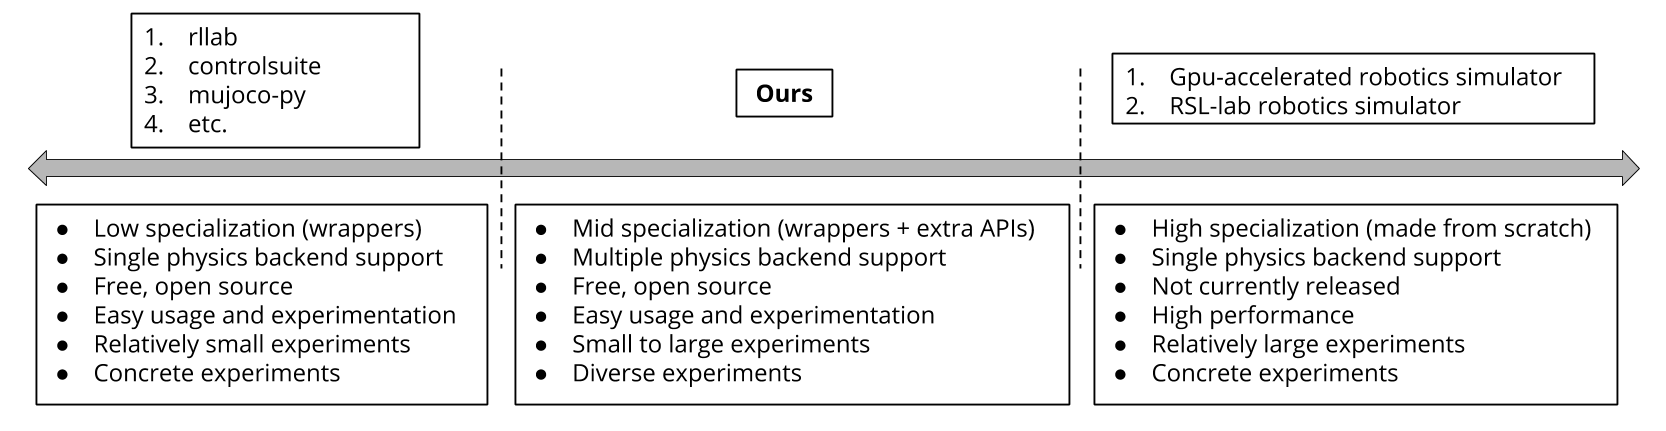
\includegraphics[width=1.0\textwidth]{./chapters/chapter_4/imgs/img_proposal_comparison.png}
        \caption{A comparison of our proposal with currently available benchmarks.}
        \label{fig:ch4_proposal_comparison}
    \end{figure}
}

As explained in chapter 1, where we presented the proposal, this thesis is mainly
focused in making a framework for evaluation of Deep Reinforcement Learning based agents
in diverse and complex environments. This chapter will give more details about the 
proposal for this thesis. We split the discussion in this chapter into the following two sections: 

\begin{itemize}
    \item Details of the proposed framework, where we discuss the core functionality 
          of the framework, the architecture to be used, and the extends of the framework.
    \item Details of the evaluation experiments, where we discuss the proposed experiments
          that will be implemented as part of this thesis.
\end{itemize}

\section{Details of the proposed framework}

The framework proposed consists basically of a multi-backend framework with exposed user APIs for task creation and configuration\todo{creation and setup tasks}. The framework is multi-backend
in the sense that it provides the user with the ability to choose to run their experiments
in a range of supported physics backends, like MuJoCo, Bullet, PhysX and FleX. We take
this approach to provide the user with more flexibility on the choice of the platform because
each backend has specific advantages and disadvantages. A description of the steps involved 
when creating a task with the proposed framework is shown in Figure @FIG-4.1, which consist of:

\begin{itemize}
    \item \textbf{User functionality} to describe the task. A description of the task is given by 
          the agents to be used, terrain generation configurations, sensors to be used, etc. This configuration
          can be passed by the user via a configuration file or programmatically.
    \item \textbf{Core functionality} used to create core data structures that will be used by the framework.
          The core data structures used involve the agents, terrain generators, sensors, and tasks. These are
          abstract in the sense that are not dependent of the specific backend (backend agnostic).
    \item \textbf{Backend-specific functionality} used to instantiate the required core representations
          into the specific resources needed for each backend. We model these are some set of \textbf{adapters}
          that can be \textbf{swapped} (dynamically loaded) depending of the choice of backend.
\end{itemize}

\figFrameworkFlow

In order to take into account the features proposed (multi-backend and diverse environment
creation) we decided to use the architecture shown in Figure @FIG-4.2. We separate the core
functionality into different modules, and create adapters for each backend (similar to wrappers) 
around the base structures in each core module. These adapters are in charge of instantiating the
necessary resources required by the base core structures. The framework then exposes the core
functionality (which is linked to the backend specific functionality) to the user via the tasks
that were created. The user can then interact with all aspects of the simulation, e.g. setting
control commands, via these created tasks.

Notice that there is a similar group of adapters that are used by the rendering backend. We
decided to take the same multi-backend approach for the visualizer because there are various situations
in which we could potentially need to choose between different rendering backends, like using a 
headless rendering backend in servers with no windowing system initialized, or using a photorealistic
rendering backend to make different experiments when trying to do more complicated simulations related to
the real world.

\figFrameworkArchitecture

\subsection{Core functionality}

The core functionality consists of the core data structures used to represent agents,
terrain and sensors, which are decoupled from the specific backends to be used. This functionality
is composed of the following components:

\begin{itemize}
    \item \textbf{Agents representations}: these representations consist of the core kinematic \todo{kinematic?} tree and its
          variants. These variants could in principle model different situations that could be needed
          for some specific task. All these representations are abstract, and their components (bodies, 
          joints, collisions, etc.) are decoupled from the specific resources provided in the backends.
          These representations are also decoupled from the specific format used to store the kinematic
          tree in disk. The formats we are considering include \textit{urdf}, \textit{mjcf}, and custom
          formats through .xml and .json files. All this functionality is summarized in Figure @FIG-4.3.

        \figFrameworkCoreAgent

    \item \textbf{Terrain representations}: these representations consist of the core terrain generator and its
          variants. These variants model the different types of terrain that one could need. In principle
          there are a few core generators, which are in charge of creating various environments. These core
          generators consist of procedural and static generators. Procedural generators are used for creating
          different terrain during runtime, and static generators are used to create a static scene and task
          with no changes in the terrain. The terrain generators will create abstract "primitives" which can then
          be used to create the desired terrain resources using the selected backend. These primitives are the minimal
          terrain resource that can be used, and consist of geometric primitives, mesh objects representing heightmaps,
          and other minimal objects that could be needed for more specific tasks. All this functionality is
          summarized in Figure @FIG-4.4.

        \figFrameworkCoreTerrain

    \item \textbf{Sensors representations}: these representations consist of the core sensors that will be exposed
          to the user in order to train an agent. These are also abstract, and get the information from the
          core agents and terrain generators. The type of sensors that will be implemented are: joint readings (angles 
          and speeds), body readings (relative position to root body, linear velocities and accelerations), 
          heightmap readings of the terrain, and camera readings in the form of RGB frames. The proposed sensors are shown
          in Figure @FIG-4.5.

        \figFrameworkCoreSensor
\end{itemize}

\subsection{Specific implementations for different backends}

%% @TODO: Talk about approach of using adapters

The backend-specific functionality is in charge of instantiating the appropiate 
resources in the given backend, like instantiating bodies and joints for the abstract 
agents, creating the appropiate terrain resources from the terrain primitives, and requesting
the sensor readings required by the abstract sensors.

The approach we chose is to use a design pattern called \textbf{bridge pattern}, which
is a pattern often used to decouple platform specific functionality from core functionality.
This approach is shown in Figure @FIG-4.6 (for the case of agents), and it basically
works as follows:

\begin{itemize}
    \item Write the core functionality (e.g. base kinematic tree agent) and any
          required variants or types. Also write base adapter code (e.g. adapters for base kinematic tree)
          which is the layer that will be exposed to the user.
    \item Use composition to wrap the core functionality with the adapter functionality.
    \item Write the required variants of the adapters corresponding to each specific backend.
          This only has to be implemented once per core functionality (e.g. one for base kinematic tree),
          and not many times for each variant that could exist.
\end{itemize}


\figBridgePattern

%% @TODO: Talk about how will everything work (dlinking)

Another detail to take into account is how to support multiple and swappable backends
for the user. To achieve this we will make use of runtime library loading. This allows us
to load the specific backend library at runtime as specified by the user, and it is an OS specific
feature usually provided in the context of dynamic linking. To fully integrate
this feature into the framework the have to ensure that the user is exposed
to \textit{base adapters}, which can then be loaded with the specific adapters using runtime loading.
This process is shown in Figure @FIG-4.7.

\figRuntimeLibraryLoading


%% @TODO: Explain about the proposed supported backends (mujoco, bullet, physx, flex)

The choice of supporting multiple backends was made because of the advantages and
disadvantages that each physics backend has. For example, PhysX 4.0 has features that
allow it to run large number of simulated agents, FleX can be used when trying to
create fluid manipulation tasks, MuJoCo can be used for more precise simulations, and
Bullet can be used for the same tasks provided by MuJoCo, but without the need to have
a license for extended usage.

\subsection{Construction and User APIs}

On top of the core functionality and the specific backend adapters explained earlier
we will implement a set of APIs that will serve for constructing a task given by the user.
These APIs will consist of the following components:

\begin{itemize}
    \item APIs for agent, terrain and sensor creation: these are high level APIs 
          that will provide the user with the functionality to create the required
          scene for a given task. This functionality will allow the user to create
          a scene programmatically, or by using configuration files. The user can then
          create a task using these APIs, or use the tasks APIs that will also be provided.
    \item APIs for task creation: these build on top of the previously mentioned APIs,
          and allow the user create experiments like: running, fetching, etc. These
          experiments will consist of the basic benchmarks we will use in our evaluation
          experiments. However, the user can still use the APIs mentioned previously to
          create new experiments.
    \item APIs for specific backend configuration: these can be used for extra configuration
          of specific backends, e.g. changing simulation properties on the fly (if supported
          by the backend). The default configurations will try to make the simulations from different
          backends as close as possible, but if extra control is needed then the user can make
          use of these APIs to configure specific experiments.
\end{itemize}

This functionality will be implemented in C/C++ in order to be as close to the backend as possible.
However, we will also provide with Python bindings for these APIs to allow the user to create and 
configure experiments through Python.

\section{Details of the proposed evaluations experiments}

A set of experiments will be set up in order to evaluate current state of the art Deep Reinforcement
Learning algorithms (like PPO, DDPG, etc.) in these new environments provided by the framework. These will consist of:

\begin{itemize}
    \item \textbf{Base Experiments}: These consist of learning environments that do not have
                                     extra functionality on top, like curricula or imitation.
                                     The idea is to test if these current state of the art 
                                     agents can solve these new environments without any extra help.

    \item \textbf{Imitation Experiments}: These consist of learning environments that have an imitation 
                                          component enabled. Only some models for some agents have the datasets
                                          from mocap data that can be used for these tasks, so these experiments will
                                          work for just a few of possible agent options. The idea is to
                                          test if by enabling imitation the agent can solve these new environments.

    \item \textbf{Curricula experiments}: These consist of learning environments that have a curriculum component
                                          enabled, e.g. increase the difficulty of a task during runtime.
                                          The idea is to test if by enabling using curriculum we can get better learning,
                                          and test different approaches to develop different curricula, and compare them as well.
\end{itemize}

%% \subsection{Adaptive curricula experiments}
%% 
%% @TODO: These experiments are some ideas that I want to ponder and see how to implement
%%        in the future. As I stated in the hypothesis, we should try some form of
%%        adaptive curricula that based on the performance of the agent it would create
%%        the terrain and task appropiately in order to encourage better learning. This
%%        would be some kind of "training-wheels" module that could be hard-coded or even 
%%        learned from experience. In my mind it sounds like and actor-supervisor approach,
%%        in which the supervisor sets the terrain generator paraeters using the provided API
%%        according to how well the agent is doing. This could be done in stages, switching between
%%        a hard-coded curricula and the adaptive curricula.

